
\RequirePackage{fix-cm}
\documentclass[]{rsos}%%%%where rsos is the template name

%% *** Do not adjust lengths that control margins, column widths, etc. ***
\usepackage{subfigure}
\usepackage{lineno}
\begin{document}

\linenumbers
%%%% Article title to be placed here
\title{Insert the article title here}

\author{%%%% Author details
Alasdair D. F. Clarke$^1$, Jess Irons$^2$, Warren James$^2$, Andrew Leber$^2$ and Amelia R Hunt$^3$}

%%%%%%%%% Insert author address here
\address{
$^{1}$Department of Psychology, University of Essex, Colchester, UK\\
$^{2}$Department of Psychology, The Ohio State Universoty, Columbus, USA\\
$^{3}$School of Psychology, University of Aberdeen, Aberdeen, UK
}

%%%% Subject entries to be placed here %%%%
\subject{Behaviour, evolution}

%%%% Keyword entries to be placed here %%%%
\keywords{visual search, optimal behaviour,
eye movements}

%%%% Insert corresponding author and its email address}
\corres{Alasdair Clarke\\
\email{a.clarke@essex.ac.uk}}

\begin{abstract}
Some abstract goes here
\end{abstract}

%%%%%%%%%% Insert the texts which can accomdate on firstpage in the tag "fmtext" %%%%%

\begin{fmtext}
%%%%%%%%%%%%%%%%%%%%%%%%%%%%
\section{Introduction}
%%%%%%%%%%%%%%%%%%%%%%%%%%%%
Hello and welcome to our paper
\end{fmtext}

\maketitle


%%%%%%%%%%%%%%%%%%%%%%%%%%%%
\section{Methods}
%%%%%%%%%%%%%%%%%%%%%%%%%%%%


\subsection{Participants}
We aim to find 64 participants to volunteer to take part in this experiment. Participants will be students from the University of Aberdeen. Some will be compensated with course credit and some will be paid \pounds 10 for their time. Sample size was determined in part due to constraints with counter-balancing; there are 16 different possible orders of tasks/conditions; we will run four participants in each order for a total of 64. All participants will sign a form giving informed consent. The study has already been approved by the University of Aberdeen Psychology Ethics Committee.

\subsection{Materials and Procedures}

The study consists of three different paradigms from the visual search literature in which large individual differences were found \cite{nowakowsak2017, irons-leber2016, kristjansson2014}. Example stimuli can be seen in Figure \ref{fig:exampleStimuli}.

\begin{figure}
\centering
\subfigure[][]{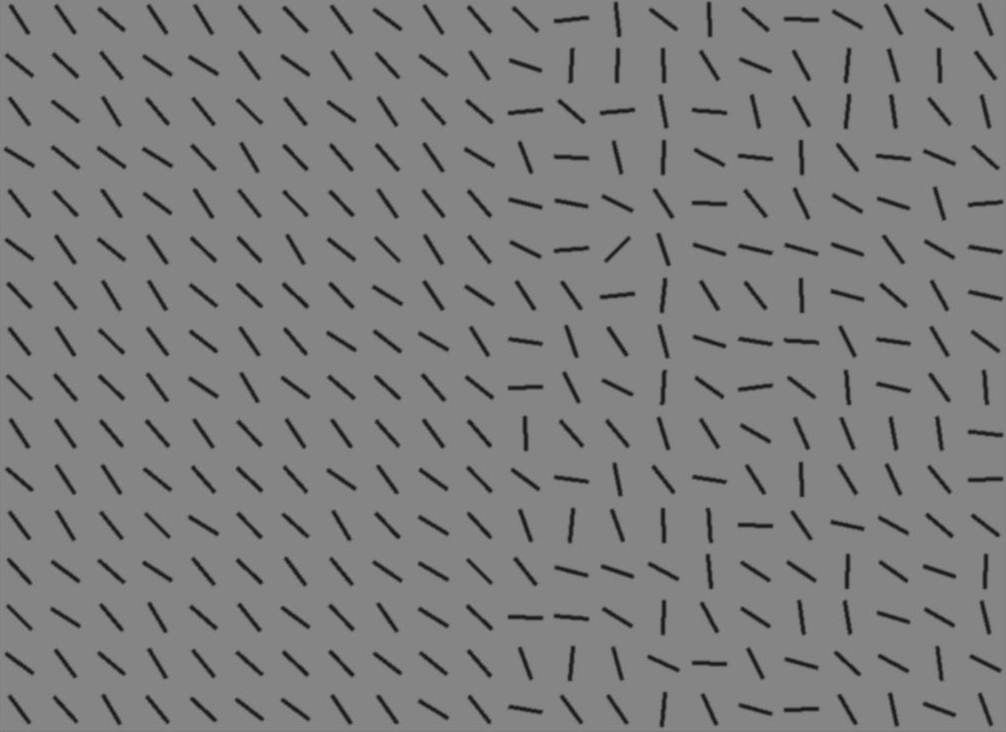
\includegraphics[height=3cm]{figures/split-half.png}}
\subfigure[][]{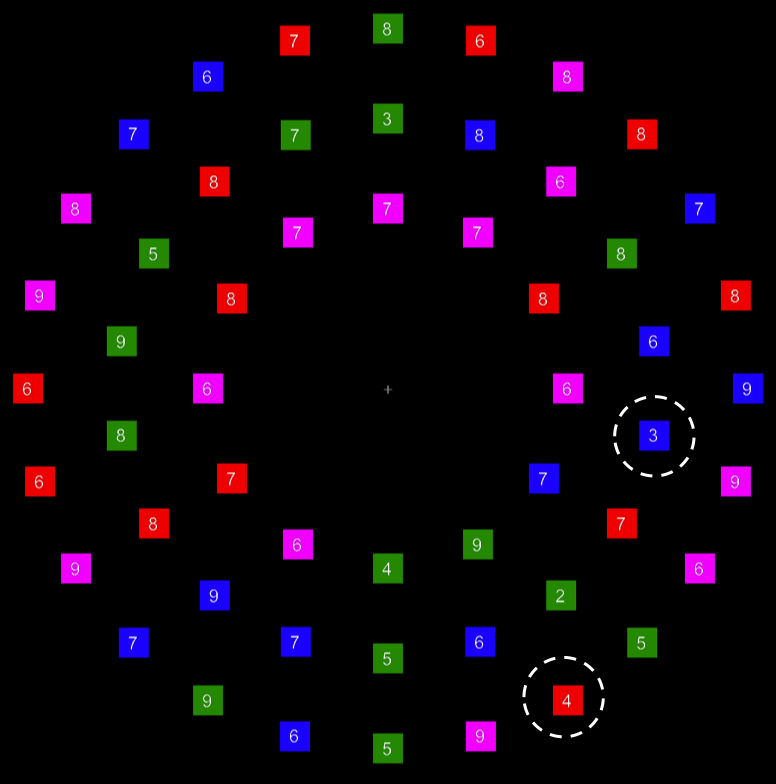
\includegraphics[height=3cm]{figures/adaptive.png}}
\subfigure[][]{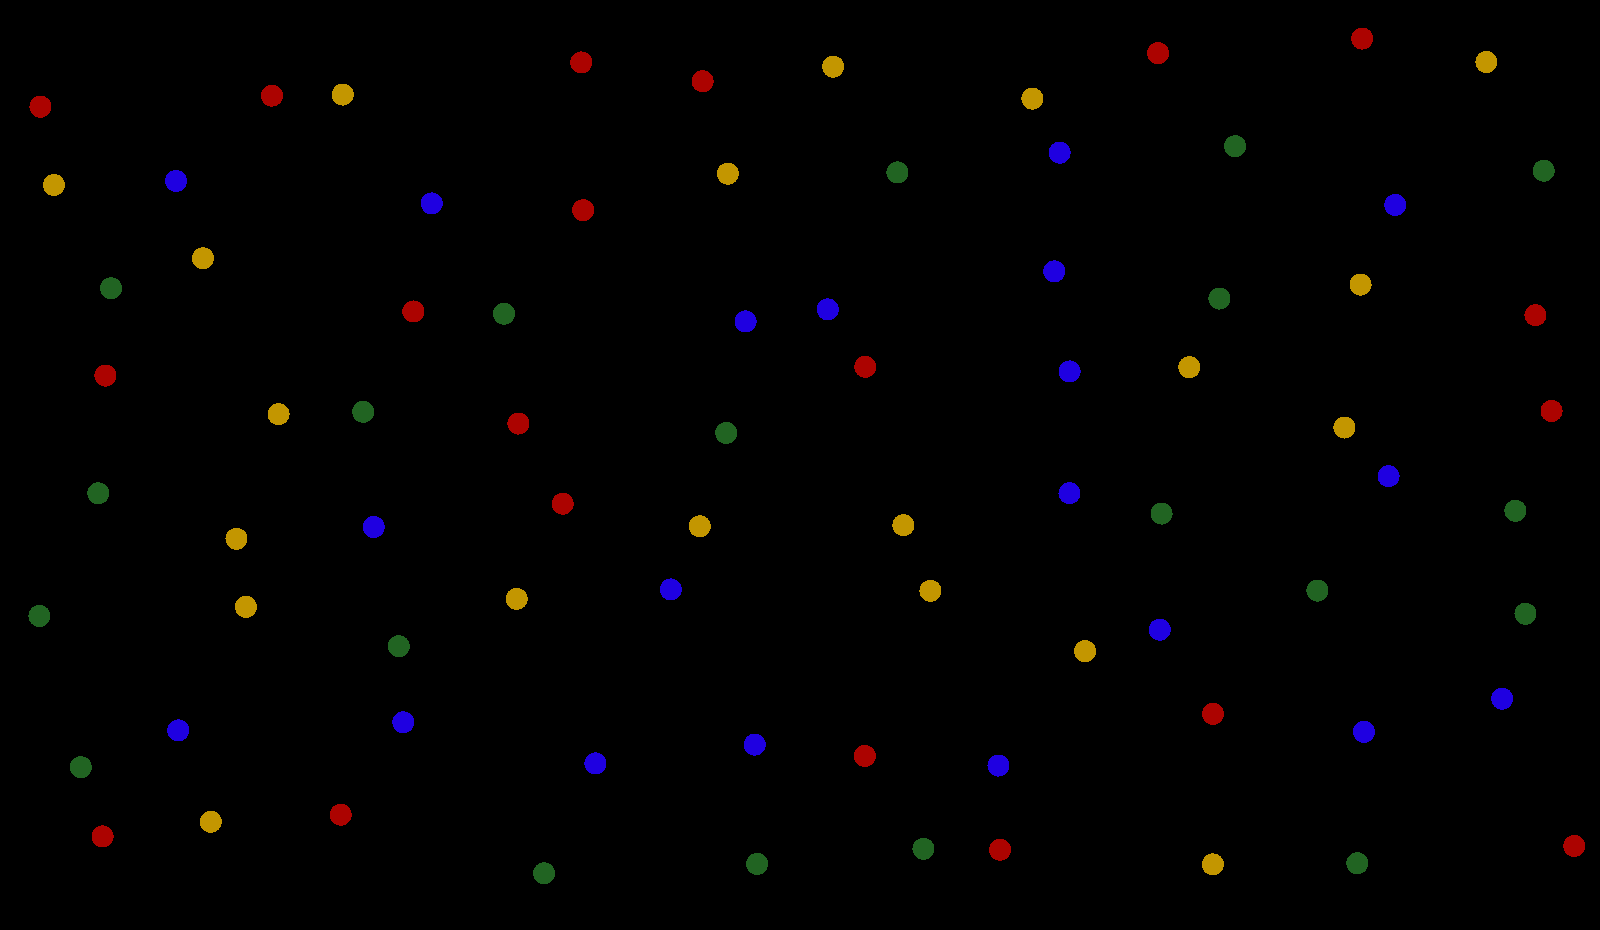
\includegraphics[height=3cm]{figures/foraging.png}}
\caption{Example stimulus from the (a) \textit{split-half}, (b) \textit{adaptive choice} and (c) \textit{foraging} paradigms}
\label{fig:exampleStimuli}
\end{figure}

The display was presented on a 17-inch CRT monitor with a resolution of $1024 \times 
768$. Stimulus generation, presentation and data collection were controlled by MATLAB and psychophysics toolbox \cite{brainard1997} run on a Powermac. 

\subsubsection{Split-half Array Search}

Stimuli consisted of arrays of black oriented line segments against a grey background. The target was oriented $45^{\circ}$ clockwise, while the distracter items had a random orientiaton with a mean of $45^{\circ}$ anti-clockwise. The varience was low (xxx) on one half of the display to create a homogeneous texture, and high (xxx) on the other side to create a heterogeneous texture. This means that when the target is present on the homogeneous side of the stimulus, it can be easily be detected with peripheral vision, but when it is in the heterogeneous half, it is much harder to detect. There were a total of xxx trials and homo- and heterogeneous sides of the display were randomly vaired from trial to trial.
 
The position of the dominant eye was recorded using a desktop-mounted EyeLink 1000 eye
tracker (SR Research, Canada) sampling eye position at 1000 Hz.
This paradigm was carried out twice to give us an estiamte of how consistent participants are in their search strategy over time. The two sessions were indentical.

\subsubsection{Attentional Control}

\subsubsection{Conjunction Foraging}

\subsection{Planned Analysis}

\subsubsection{Split-half array search}

In order to characterise an individual's behaviour in this task, we will compute the proportion of the first $n$ fixations that were on heterogeneous (difficult) side of the stimuli, over all target absent trials\footnote{Only take correct trials?}. \cite{nowakowsak2017} demonstrated a strong correlation between an this metric (for $n=5$) and reaction times ($r=$). However, a re-analysis of their data shows that an even stronger correlation is obtained with $n=3$.



\subsubsection{Attentional Control}

Following \cite{irons-leber2016}, individual differences will be characterized using two measures:\\
1) Proportion of optimal choices on plateaus. An optimal choice is defined as responding to whichever of the two target colours has the fewest items in the display. This will be based on correct plateau trials only. \\ 
2) Switching frequency. Switching is defined as responding to a different target color on trial $N$+1 than on trial $N$, and is presented as a proportion of the total number of trials (excluded incorrect trials, the trial after an incorrect trial, and the first trial of each block).\\
Both measures have been shown to correlate with overall RT in previous experiments (Proportion Optimal $r$=-.56, $p$<.001; Switch Frequency $r$=.45, $p$=.001; based on $N$=50 and using the same number of trials as in the current experiment). As additional validation, correlational analyses between both measures and RT will also be conducted in the current experiment.

\subsubsection{Conjunction Foraging}

Data analysis will follow \cite{kristjansson2014} and Johannesson et al. (2016). The main measure of interest will be the average run length per trial. A run is defined as a succession of one or more of the same target type which is followed and preceded by the other target type or no target. The average length is the average number of consecutive target selections per run. As with the other experiments, we will also measure the average response (time to select the final target on correct trials).

\subsubsection{}


\subsection{Exploratory Analysis}

We will carry out additional analysis, above and beyond what has been documented above, but the exact nature of this will be contingent on the nature of the results. Something like PCA may be interesting. 

%%%%%%%%%%%%%%%%%%%%%%%%%%%%
\section{Results}
%%%%%%%%%%%%%%%%%%%%%%%%%%%%

\subsection{Split-half Array Search}
Our results are broadly in line with \cite{nowakowsak2017}. The correlation between accuracy and reaction times between the two sessions is shown in Figure \ref{fig:splithalf_summary}(a, b). We can clearly see that there are large differences from one participant to the next in terms of both the proportion of hard targets found, and reading times. Furthermore, test-retest reliability appears to be reasonable, with correlations of around $r = 0.78$ (the value of $r = 0.71$ or easy targets is slightly lower, likely due to the restricted range).

\begin{figure}
\centering
\subfigure[][]{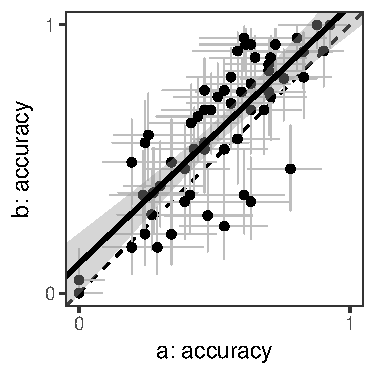
\includegraphics[width=5cm]{../Scripts/lineseg/scratch/acc_correlation.pdf}}
\subfigure[][]{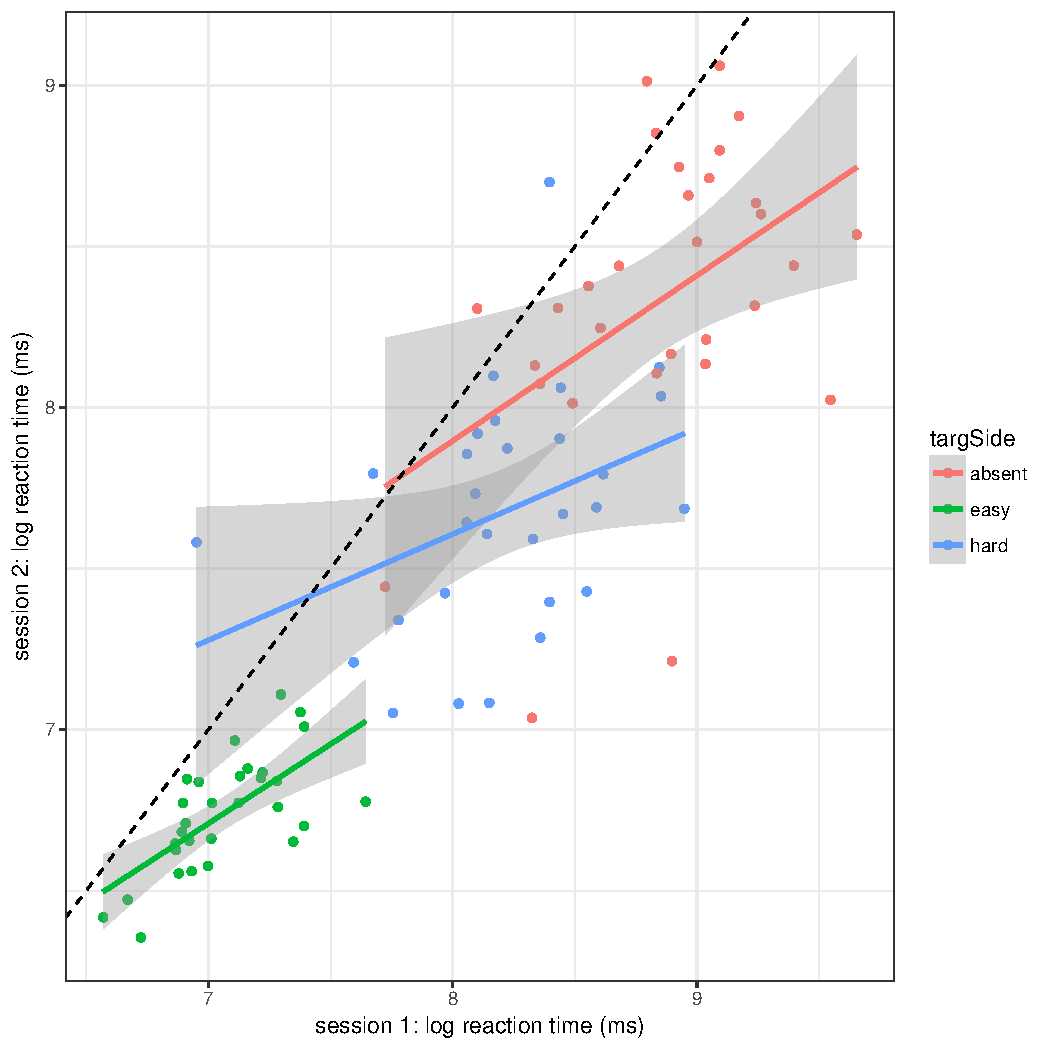
\includegraphics[width=5cm]{../Scripts/lineseg/scratch/rt_correlation.pdf}}
\subfigure[][]{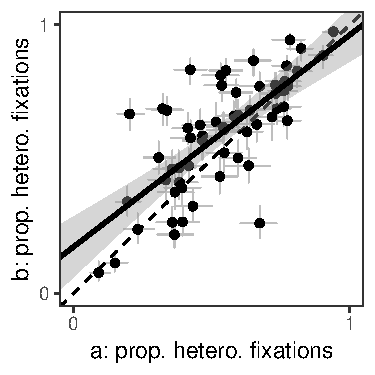
\includegraphics[width=5cm]{../Scripts/lineseg/scratch/strat_corr.pdf}}
\subfigure[][]{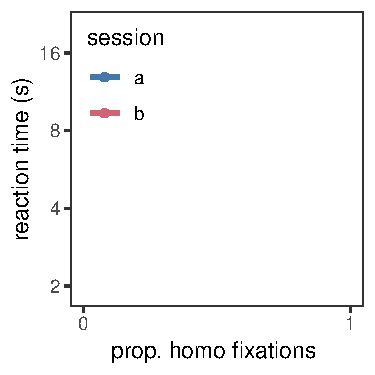
\includegraphics[width=5cm]{../Scripts/lineseg/scratch/strat_compare_meanlog_rt.pdf}}
\caption{Correlation between the two sessions of the \textit{split-half} paradigm for (a)  accuracy (TP-heterogeneous), (b) reaction times and (c) search strategy. (d) initial search strategy correlates with reaction times in both sessions. Each point represents a participant and the error-bars indicate 95\% confidence intervals.}
\label{fig:splithalf_summary}
\end{figure}

We can also look at the initial search strategies adopted by our participants \ref{fig:splithalf_summary}(c, d). Again, we see large and stable individual differences across the two sessions. More importantly, as with \cite{nowakowsak2017}, we see that the search strategies give a good correlation with reaction times. 


\subsection{Adaptive Choice}

\subsubsection{Conjunction Foraging}


%%%%%%%%%%%%%%%%%%%%%%%%%%%%
\section{Discussion}
%%%%%%%%%%%%%%%%%%%%%%%%%%%%



\bibliographystyle{plain}
\bibliography{literature}

\end{document}


